% Options for packages loaded elsewhere
\PassOptionsToPackage{unicode}{hyperref}
\PassOptionsToPackage{hyphens}{url}
%
\documentclass[
]{article}
\usepackage{amsmath,amssymb}
\usepackage{iftex}
\ifPDFTeX
  \usepackage[T1]{fontenc}
  \usepackage[utf8]{inputenc}
  \usepackage{textcomp} % provide euro and other symbols
\else % if luatex or xetex
  \usepackage{unicode-math} % this also loads fontspec
  \defaultfontfeatures{Scale=MatchLowercase}
  \defaultfontfeatures[\rmfamily]{Ligatures=TeX,Scale=1}
\fi
\usepackage{lmodern}
\ifPDFTeX\else
  % xetex/luatex font selection
\fi
% Use upquote if available, for straight quotes in verbatim environments
\IfFileExists{upquote.sty}{\usepackage{upquote}}{}
\IfFileExists{microtype.sty}{% use microtype if available
  \usepackage[]{microtype}
  \UseMicrotypeSet[protrusion]{basicmath} % disable protrusion for tt fonts
}{}
\makeatletter
\@ifundefined{KOMAClassName}{% if non-KOMA class
  \IfFileExists{parskip.sty}{%
    \usepackage{parskip}
  }{% else
    \setlength{\parindent}{0pt}
    \setlength{\parskip}{6pt plus 2pt minus 1pt}}
}{% if KOMA class
  \KOMAoptions{parskip=half}}
\makeatother
\usepackage{xcolor}
\usepackage[margin=1in]{geometry}
\usepackage{graphicx}
\makeatletter
\def\maxwidth{\ifdim\Gin@nat@width>\linewidth\linewidth\else\Gin@nat@width\fi}
\def\maxheight{\ifdim\Gin@nat@height>\textheight\textheight\else\Gin@nat@height\fi}
\makeatother
% Scale images if necessary, so that they will not overflow the page
% margins by default, and it is still possible to overwrite the defaults
% using explicit options in \includegraphics[width, height, ...]{}
\setkeys{Gin}{width=\maxwidth,height=\maxheight,keepaspectratio}
% Set default figure placement to htbp
\makeatletter
\def\fps@figure{htbp}
\makeatother
\setlength{\emergencystretch}{3em} % prevent overfull lines
\providecommand{\tightlist}{%
  \setlength{\itemsep}{0pt}\setlength{\parskip}{0pt}}
\setcounter{secnumdepth}{-\maxdimen} % remove section numbering
% definitions for citeproc citations
\NewDocumentCommand\citeproctext{}{}
\NewDocumentCommand\citeproc{mm}{%
  \begingroup\def\citeproctext{#2}\cite{#1}\endgroup}
\makeatletter
 % allow citations to break across lines
 \let\@cite@ofmt\@firstofone
 % avoid brackets around text for \cite:
 \def\@biblabel#1{}
 \def\@cite#1#2{{#1\if@tempswa , #2\fi}}
\makeatother
\newlength{\cslhangindent}
\setlength{\cslhangindent}{1.5em}
\newlength{\csllabelwidth}
\setlength{\csllabelwidth}{3em}
\newenvironment{CSLReferences}[2] % #1 hanging-indent, #2 entry-spacing
 {\begin{list}{}{%
  \setlength{\itemindent}{0pt}
  \setlength{\leftmargin}{0pt}
  \setlength{\parsep}{0pt}
  % turn on hanging indent if param 1 is 1
  \ifodd #1
   \setlength{\leftmargin}{\cslhangindent}
   \setlength{\itemindent}{-1\cslhangindent}
  \fi
  % set entry spacing
  \setlength{\itemsep}{#2\baselineskip}}}
 {\end{list}}
\usepackage{calc}
\newcommand{\CSLBlock}[1]{\hfill\break\parbox[t]{\linewidth}{\strut\ignorespaces#1\strut}}
\newcommand{\CSLLeftMargin}[1]{\parbox[t]{\csllabelwidth}{\strut#1\strut}}
\newcommand{\CSLRightInline}[1]{\parbox[t]{\linewidth - \csllabelwidth}{\strut#1\strut}}
\newcommand{\CSLIndent}[1]{\hspace{\cslhangindent}#1}
\ifLuaTeX
  \usepackage{selnolig}  % disable illegal ligatures
\fi
\usepackage{bookmark}
\IfFileExists{xurl.sty}{\usepackage{xurl}}{} % add URL line breaks if available
\urlstyle{same}
\hypersetup{
  pdftitle={Assessing the effects of temperature on backswimmer development and dispersal},
  pdfauthor={Nicole Regimbal},
  hidelinks,
  pdfcreator={LaTeX via pandoc}}

\title{Assessing the effects of temperature on backswimmer development
and dispersal}
\author{Nicole Regimbal}
\date{September 25, 2025}

\begin{document}
\maketitle

\section{Introduction}\label{introduction}

Rising global temperatures is forcing many species to shift their range
distributions to track suitable climatic conditions (Chen et al. 2011).
The ability of a species to successfully do so is largely dependent on
dispersal (Berg et al. 2010), movement away from an organisms natal
habitat which connects discrete populations. If a species is unable to
respond to climate change through dispersal, they must adapt to higher
temperatures or will face extinction (Berg et al. 2010). Dispersal is a
two-fold behavior, shaped by both dispersal ability (the physical and
physiological ability to disperse) and dispersal propensity (the
motivation to disperse). Dispersal ability can be treated as a
foundation for the extent to which dispersal is possible. Dispersal
propensity builds upon this foundation, if there is a physical capacity
to disperse then an individual may or may not be motivated to do so,
shaping the observed dispersal behavior (Steyn et al. 2016). Dispersal
propensity may increase with temperature (Franzén and Nilsson 2012);
however, dispersal ability and dispersal propensity can conflict with
each other. when dispersal ability is impeded the independent effects of
temperature on dispersal propensity cannot be expressed. Therefore,
isolating the impacts of temperature on dispersal ability is important
to understand changes in dispersal trends with temperature, elucidating
the extent to which dispersal is possible and motivated.

Temperature can alter dispersal ability through developmental and
physiological changes that affect fitness. High temperatures typically
increase metabolic rate and respiration, resulting in smaller body size
(Sheridan and Bickford 2011). The impact of temperature on metabolic
rate is especially apparent in ectotherms (Dillon et al. 2010),
organisms which rely on external temperature to regulate body
temperature. Understanding the effects of temperature on dispersal
ability is important to determine how the distribution and abundance of
populations may change.

In this study, we experimentally assessed the impacts of temperature on
the development and dispersal ability in backswimmers (\emph{Notonecta
undulata}). Backswimmers are common semi-aquatic insects found in
freshwater throughout North America and can facultatively disperse via
flight (Clark 1928). Currently, there is no research to our knowledge
that connects temperature to dispersal in backswimmers. We raised
juvenile backswimmers in different temperatures during development then
conducted a dispersal assay. We predicted that 1) high temperatures will
increase backswimmer mortality, 2) high temperatures will lower body
condition, and 3) the effects of temperature on body condition will
determine dispersal rates. Our study is the first, to our knowledge, to
collect long-term data on the impacts of temperature on backswimmers.
Understanding the impacts of temperature on development is important to
predict how population sizes and distributions are going to change as
global temperatures rise.

\section{Methods}\label{methods}

\subsection{Field Collection}\label{field-collection}

Juvenile backswimmers for this project were opportunistically collected
from ponds at the University of Toronto's Koffler Scientific Reserve
field station. Only 2nd instar (out of 5 total instars) backswimmers
were used to enter the temperature-manipulative experiment. We filtered
through all collected backswimmers for 2nd instars using size matching.
This project used sample size was 350 2nd instar backswimmers. Due to
sampling effort constraints, backswimmmers were added to the experiment
in 5 blocks on consecutive days to allow for the continuous sampling.

\subsection{Experimental Design}\label{experimental-design}

This project consists of two consecutive experiments. First, we assess
the effects of temperature on backswimmer fitness (survival,
developmental rate, body condition). Then, individuals that successfully
survived to adulthood entered a dispersal assay; we related temperature
during development and body condition to dispersal behaviors.

We manipulated water temperature using aquaria heaters in 35 20-gallon
mesocosms. We used 5 temperature treatments: 22°C, 24°C, 26°C, 28°C, and
30°C. Higher temperatures are often associated with higher mortality,
thus we varied the number of replicates by temperature treatment with
the goal of having a sufficient sample size of adult backswimmers at
high temperatures to conduct the dispersal assay. We included 5
replicates of the 22°C treatment, 6 replicates of the 24°C treatment, 7
replicates of the 26°C treatment, 8 replicates of the 28°C treatment,
and 9 replicates of the 30°C treatment (35 total mesocosms). We used
aquarium bubblers to homogenize the temperature throughout the mesocosms
and full-spectrum LED overhanging lights were placed above the mesocosms
to mimic natural sunlight with 12 hour on-off increments. In these
mesocosms, backswimmers were separated into individual cups to expose
them to the temperature treatment without interacting with conspecifics,
which would introduce competition and cannibalism. 10 individual
backswimmers were randomly assigned to each mesocosm. We fed the
backswimmers zooplankton \emph{ad libitum} throughout the experiment.

\subsubsection{\texorpdfstring{\emph{Temperature on
development}}{Temperature on development}}\label{temperature-on-development}

Every day of the experiment, we assessed backswimmer survival and
development. Backswimmers molt to develop into the next instar, leaving
a shedded exoskeleton intact. When a backswimmer molted, we removed the
exoskeleton and recorded the day the molt occurred for that individual.
Additionally, after recording survival, dead backswimmers were removed
from the experiment.

If a backswimmer survived to adulthood, we recorded the date they molted
into an adult and removed them from the temperature treatment. We
measured the thorax width (mm) of the backswimmer using a caliper.
Additionally, we allowed the backswimmer to dry before recording the
mass (g). Body condition is calculated as thorax width (mm)/mass (g).

\subsubsection{\texorpdfstring{\emph{Dispersal
assay}}{Dispersal assay}}\label{dispersal-assay}

Adult backswimmers acclimated to ambient temperatures over 10 days to
allow their hemelytra to harden so they can fly. This also isolates the
effect of temperature on development and dispersal ability rather than
temperature shock (from moving individuals directly from the temperature
treatment to dispersal assay) on dispersal. The dispersal assay was
conducted in two parts: dispersal count and absolute dispersal.
Dispersal assays were conducted outside on sunny days because
backswimmers require a light cue to disperse (CITE).

Dispersal count reflects the dispersal propensity of the backswimmer.
Individual backswimmer cups were loosely covered with clear plastic
wrap. Backswimmers are exposed to the light cue so can attempt to
disperse, but are not able to leave the cup. Thus, backswimmers can
attempt to disperse multiple times. We recorded the number of times in a
15-minute window that the backswimmer attempted to disperse. We followed
this with an absolute dispersal assay for which the plastic wrap was
removed. Backswimmers were given 3 hours to disperse from their cups
before their dispersal state (0 = stayed, 1 = dispersed) was recorded.

\subsection{Data Analysis}\label{data-analysis}

All statistical analyses were conducted using R Statistical Software
version 4.3.1. We confirmed all models met assumptions using the DHARMa
package in R. We assessed how temperature influenced survival using a
generalized linear mixed effects model (GLMM) with the binomial error
structure using the lme4 package (Bates et al. 2014). This model treated
survival as a binomial response variable, with the fixed effect of
temperature and the random effect of mesocosm nested in block. We
assessed how temperature affects the speed at which an individual molts
by calculating the molt rate as the number of molts divided by the
number of days an individual survived (or reached adulthood). We
assessed molt rate by conducting a linear mixed effects model with
temperature as a fixed effect and mesocosm nested in block as a random
effect. Additionally, we conducted a linear mixed effects model to
assess body condition, using body condition as the response variable,
temperature as the fixed effect, and mesocosm nested in block as the
random effect. We assessed dispersal count and absolute dispersal in
separate GLMMS with a poisson distribution and a binomial distribution,
respectively. In both models, temperature and body condition will be
fixed effects and mesocosm nested in block will be a random effect.

\section{Results}\label{results}

We found that temperature has a significant negative effect on
backswimmer survival (\emph{p} \textless{} 0.001). Survival was
generally low across all treatments (Figure 1). The highest survival was
in the 22°C treatment, with a fitted survival probability of 0.28. No
backswimmers in the 30°C treatment survived to adulthood. In the 22°C
treatment 14 individuals survived to adulthood, in the 24°C treatment 20
individuals survived to adulthood, in the 26°C treatmnet 10 individuals
survived to adulthood, and in the 28°C treatment 4 individuals survived
to adulthood. Temperature significantly increased molt rate (\emph{p}
\textless{} 0.001) such that mean molt rate increased from 0.079 at 22°C
to 0.17 at 30°C. When individuals molted faster, the odds of survival
significantly decreased (\emph{p} \textless{} 0.001, Figure 2).

\begin{figure}
\centering
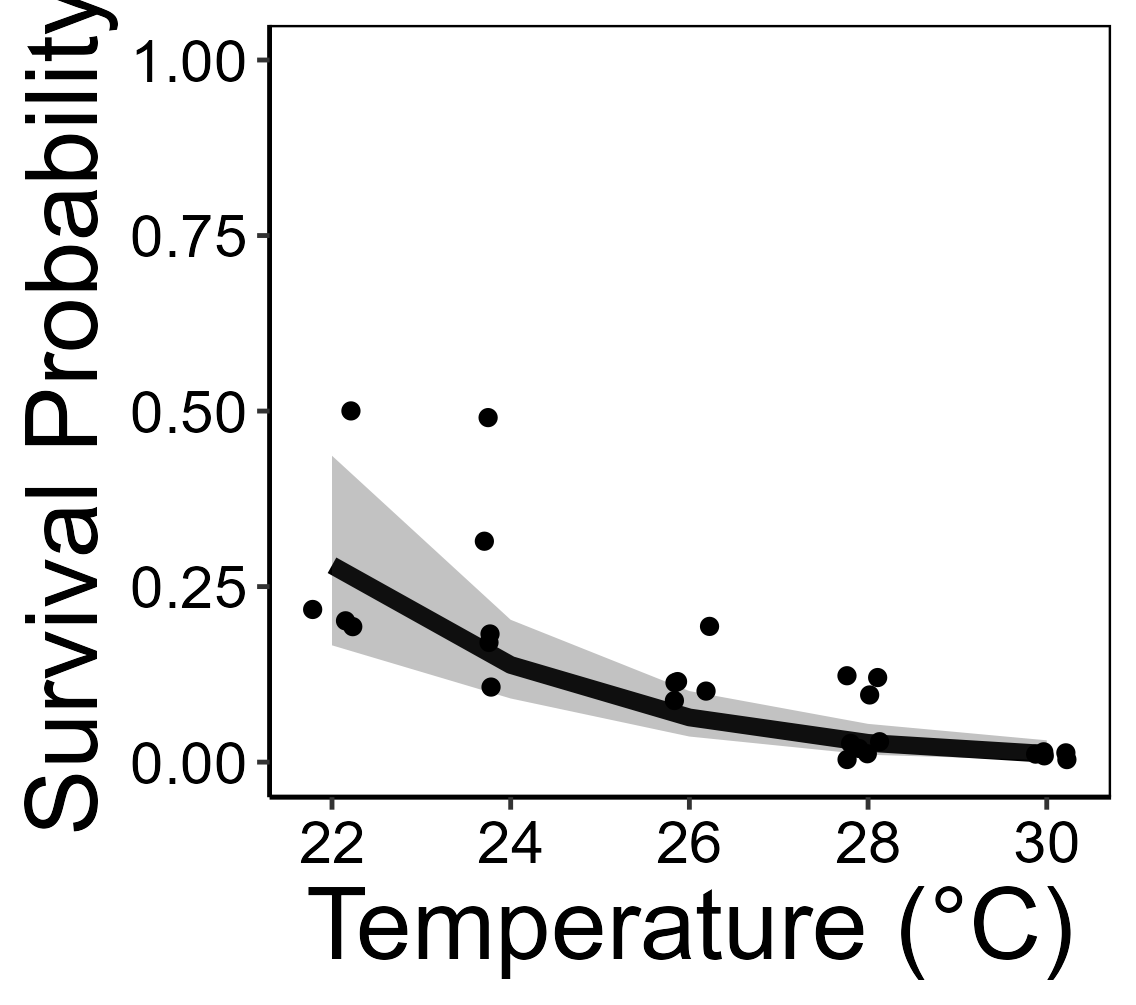
\includegraphics[width=0.5\textwidth,height=\textheight]{../03_figs/survival_plot.png}
\caption{Survival probability +/-95\% CI of juvenile backswimmers as a
function of temperature. Temperature has a negative effect on survival.}
\end{figure}

\begin{figure}
\centering
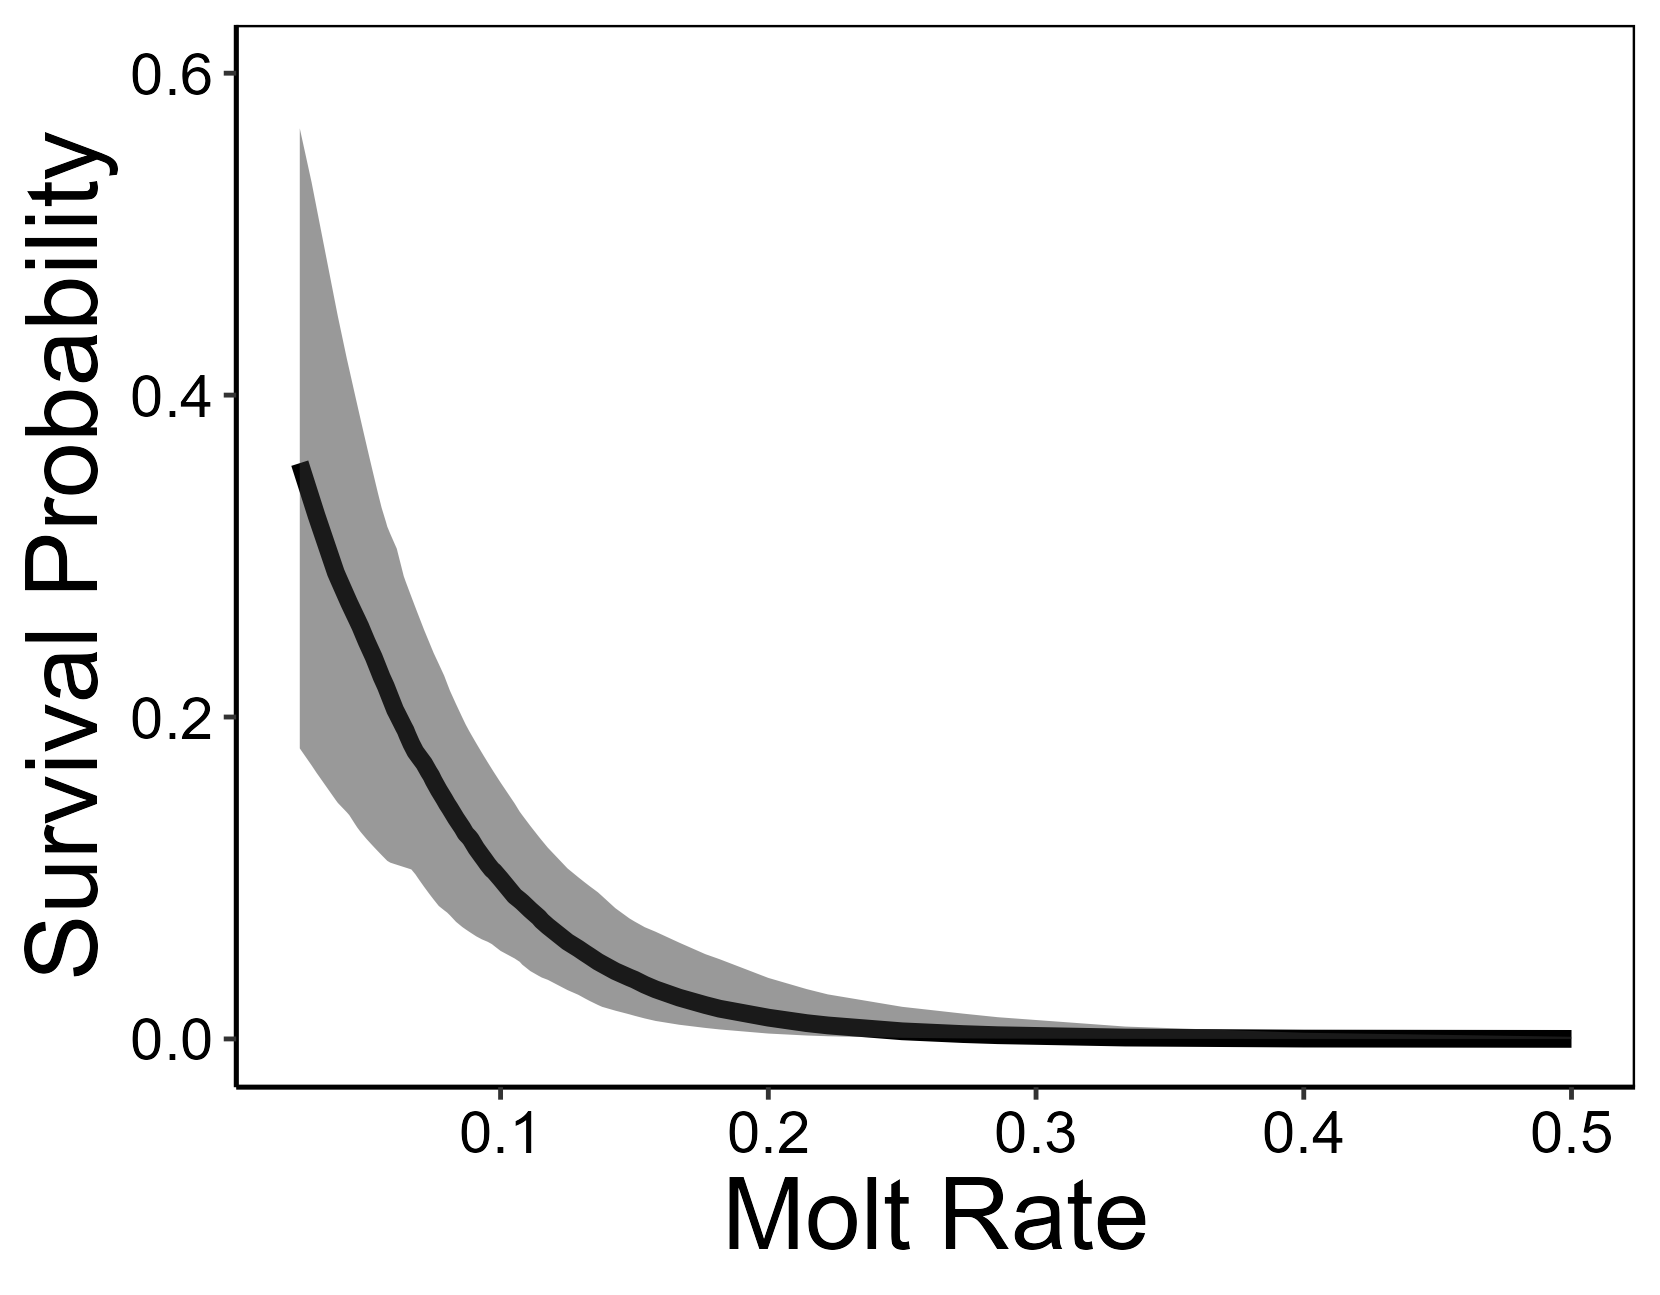
\includegraphics[width=0.5\textwidth,height=\textheight]{../03_figs/moltrate_survival_plot.png}
\caption{Survival probability +/-95\% CI of juvenile backswimmers as a
function of molt rate. Individuals that molt faster are less likely to
survive.}
\end{figure}

We did not find a significant effect of temperature on body condition.
It is important to note that due to high mortality in the experiment
this analysis lacked power due to sample size (n = 48). Only 30 of those
adults survived to the dispersal assay. There were only 3 dispersal
attempts in the dispersal count assay. Only 1 individual dispersed in
the absolute dispersal assay. Due to these extremely low dispersal rates
we were not able to statistically detect the impacts of temperature and
body condition on dispersal.

\section{Discussion}\label{discussion}

We outline the effects of rising temperatures on \emph{N. undulata}
development. Survival was low overall in the experiment across all
treatments. However, in nature juvenile survival probability is also
quite low due to many selective factors such as competition, predation,
and cannibalism from conspecifics (Hungerford 1934). These pressures
filter individuals such that only the most fit and resilient survive. In
our experiment we remove all these selective pressures by individually
separating the backswimmers from each other and feeding them
individually. In this way, we likely raised many backswimmers that would
not have survived in nature either, so low survival across treatments is
expected. Still, we can compare the relative differences between
treatments to understand the impacts of temperature on survival.

At high temperatures, backswimmers molted more frequently which
correlated with low survival at high temperatures (Figure 2). Molting is
an energetically intensive process (Tessier et al. 1983); when there is
less time between molts individuals may be less able to accumulate
sufficient biomass (Stamp 1990). Metabolic rate is also higher at high
temperatures, resulting in increased energy expenditure (Dillon et al.
2010). The combined effects of a smaller period to accumulate biomass in
conjunction with increased energy expenditure increases the risks of
molting at high temperatures.

Interestingly, we observed nearly no dispersal in our experiments. We
identify some potential interpretations of these patterns. First,
temperature may simply not affect dispersal. However, even if
temperature has no effect, we still expect that some baseline of
individuals will disperse. Small amounts of water are not long-term
suitable conditions for backswimmers, so when placed outside and exposed
to a light cue we expect that individuals which can disperse would do so
to find more suitable habitat. The near complete lack of dispersal
suggests some other mechanism may be driving these results. Another
potential reason for the lack of dispersal is that individuals lack the
ability to do so. Backswimmers are voracious predators in their natural
habitats (Clark 1928) which require good body condition to disperse
(Baines et al. 2015). Though we expect it to be more difficult for
individuals in high temperatures to build energy reserves requiring more
consumption (Ingram and Burns 2018), individuals may not have been able
to build sufficient energy reserves to disperse regardless of
temperature. Another explanation may be related to dispersal propensity.
Environmentally, dispersal propensity was likely low due to a lack of
competition, cannibalism, or predation. To minimize the effects of
temperature on dispersal propensity, backswimmers were removed from
their temperature treatments as adults for a minimum of 10 days. Thereby
removing the effects of temperature and temperature shock (an abrupt
change from the temperature treatment to ambient temperature) on
dispersal. Thus, we may not have been able to evaluate dispersal ability
due to such minimal dispersal propensity.

Researching the foundational impacts of temperature on development is
important to understand species' dispersal patterns. These behaviors are
important in dictating the fate of species' range persistence as global
temperatures rise. Especially in highly heterogenous landscapes, the
configuration of suitable patches and the species' dispersal ability
will determine whether species can successfully track their range
(Anderson et al. 2012). Thus, this may be especially apparent in aquatic
systems, where conditions such as size and water quality influence local
temperatures regardless of air temperature (Dallas 2011). Since we
observed that body condition can recover when backswimmers move from
high to ambient temperatures, this heterogeneity in the landscape may
increase the benefits of dispersing since temperature variability is not
necessarily related to dispersal distance. We have recorded important
temperature-dependent developmental parameters that can be used in
future research on backswimmer thermal performance.

\section*{References}\label{references}
\addcontentsline{toc}{section}{References}

\phantomsection\label{refs}
\begin{CSLReferences}{1}{0}
\bibitem[\citeproctext]{ref-andersonImmigrantsRefugeesImportance2012}
Anderson, A. S., A. E. Reside, J. J. VanDerWal, L. P. Shoo, R. G.
Pearson, and S. E. Williams. 2012.
\href{https://doi.org/10.1111/j.1365-2486.2012.02683.x}{Immigrants and
refugees: The importance of dispersal in mediating biotic attrition
under climate change}. Global Change Biology 18:2126--2134.

\bibitem[\citeproctext]{ref-bainesDispersalDependsBody2015}
Baines, C. B., S. J. McCauley, and L. Rowe. 2015.
\href{https://doi.org/10.1002/ece3.1508}{Dispersal depends on body
condition and predation risk in the semi-aquatic insect, {Notonecta}
undulata}. Ecology and Evolution 5:2307--2316.

\bibitem[\citeproctext]{ref-batesFittingLinearMixedEffects2014}
Bates, D., M. Mächler, B. Bolker, and S. Walker. 2014, June.
\href{https://arxiv.org/abs/1406.5823}{Fitting {Linear Mixed-Effects
Models} using Lme4}. arXiv.

\bibitem[\citeproctext]{ref-bergAdaptDisperseUnderstanding2010}
Berg, M. P., E. T. Kiers, G. Driessen, M. Van Der Heijden, B. W. Kooi,
F. Kuenen, M. Liefting, H. A. Verhoef, and J. Ellers. 2010.
\href{https://doi.org/10.1111/j.1365-2486.2009.02014.x}{Adapt or
disperse: Understanding species persistence in a changing world}. Global
Change Biology 16:587--598.

\bibitem[\citeproctext]{ref-chenRapidRangeShifts2011}
Chen, I.-C., J. K. Hill, R. Ohlemüller, D. B. Roy, and C. D. Thomas.
2011. \href{https://doi.org/10.1126/science.1206432}{Rapid {Range
Shifts} of {Species Associated} with {High Levels} of {Climate
Warming}}. Science 333:1024--1026.

\bibitem[\citeproctext]{ref-clarkSeasonalDistributionLife1928}
Clark, L. B. 1928. \href{https://doi.org/10.2307/1929407}{Seasonal
{Distribution} and {Life History} of {Notonecta Undulata} in the
{Winnipeg Region}, {Canada}}. Ecology 9:383--403.

\bibitem[\citeproctext]{ref-dallasMicroscaleHeterogeneityWater2011}
Dallas, H. F. 2011.
\href{https://doi.org/10.10520/EJC116810}{Micro-scale heterogeneity in
water temperature}. Water SA 37:505--512.

\bibitem[\citeproctext]{ref-dillonGlobalMetabolicImpacts2010}
Dillon, M. E., G. Wang, and R. B. Huey. 2010.
\href{https://doi.org/10.1038/nature09407}{Global metabolic impacts of
recent climate warming}. Nature 467:704--706.

\bibitem[\citeproctext]{ref-franzenClimatedependentDispersalRates2012}
Franzén, M., and S. G. Nilsson. 2012.
\href{https://doi.org/10.1007/s10841-012-9481-4}{Climate-dependent
dispersal rates in metapopulations of burnet moths}. Journal of Insect
Conservation 16:941--947.

\bibitem[\citeproctext]{ref-hungerfordGenusNotonectaWorld1934}
Hungerford, H. B. 1934. The genus {Notonecta} of the {World}
({Notonectidae-Hemiptera}). University of Kansas Science Bulletin.

\bibitem[\citeproctext]{ref-ingramTopdownControlAquatic2018}
Ingram, T., and Z. D. Burns. 2018.
\href{https://doi.org/10.1002/ece3.4367}{Top-down control by an aquatic
invertebrate predator increases with temperature but does not depend on
individual behavioral type}. Ecology and Evolution 8:8256--8265.

\bibitem[\citeproctext]{ref-sheridanShrinkingBodySize2011}
Sheridan, J. A., and D. Bickford. 2011.
\href{https://doi.org/10.1038/nclimate1259}{Shrinking body size as an
ecological response to climate change}. Nature Climate Change
1:401--406.

\bibitem[\citeproctext]{ref-stampGrowthMoltingTime1990}
Stamp, N. E. 1990. \href{https://doi.org/10.1007/BF00318541}{Growth
versus molting time of caterpillars as a function of temperature,
nutrient concentration and the phenolic rutin}. Oecologia 82:107--113.

\bibitem[\citeproctext]{ref-steynDispersalPropensityNot2016}
Steyn, V. M., K. A. Mitchell, and J. S. Terblanche. 2016.
\href{https://doi.org/10.1098/rspb.2016.0905}{Dispersal propensity, but
not flight performance, explains variation in dispersal ability}.
Proceedings of the Royal Society B: Biological Sciences 283:20160905.

\bibitem[\citeproctext]{ref-tessierStarvationDaphniaEnergy1983}
Tessier, A. J., L. L. Henry, C. E. Goulden, and M. W. Durand. 1983.
\href{https://doi.org/10.4319/lo.1983.28.4.0667}{Starvation in
{Daphnia}: {Energy} reserves and reproductive Allocation1}. Limnology
and Oceanography 28:667--676.

\end{CSLReferences}

\end{document}
